\documentclass{assignment}

\course{ECO 120-04}
\name{Lucas Reddinger}
\date{Monday 5 December 2022}
\doctitle{Assignment 13: Monetary exchange}

\begin{document}
\RaggedRight

\beginassignment{}

\emph{Due Friday 9 December.} Please submit hardcopy at the beginning of class (11:00 a.m.), or if you prefer, under the door of Wimberly Hall 339C by 10:50 a.m.

\section{International trade}

\begin{enumerate}

\item Is a depreciation of the U.S.~dollar a good thing or a bad thing for the United States? Explain.

\vspace{5.0\baselineskip}

\item Suppose Brazil experiences a severe recession which results in high unemployment and low incomes.
Describe the impact on international trade between Brazil and Argentina, one of its major trading
partners, and describe and illustrate the impact on the exchange rate between the Brazilian Real and
the Argentine Peso.

\vfill

\clearpage

\item Suppose interest rates increase in both European countries that use the Euro and the United Kingdom,
whose currency is the British Pound. Suppose that the increase in interest rate in the United Kingdom
was larger. Illustrate and describe the impact on the U.K.~Pound (GBP) / Euro (EUR) exchange rate.
Does the Pound appreciate or depreciate? Does the Euro appreciate or depreciate? What happens
to the quantity of trading between two currencies?

\vfill

\item Suppose there is an increase in the average level of income in the United States, while the average
level of income stays the same in countries that use the Euro as their currency.

\begin{enumerate}

\item Describe and illustrate the impact on the exchange rate between U.S.~dollars and Euros.

\vfill

\item Did the U.S.~dollar appreciate, depreciate or neither? Did the Euro appreciate, depreciate or
neither? Was the change in the exchange rate associated with a good thing or a bad thing for
the United States?

\vspace{3.0\baselineskip}

\end{enumerate}

\clearpage

\item Suppose there is an increase in demand among European countries (that use the Euro) for information
technology services produced in the United States.

\begin{enumerate}

\item Describe and illustrate the impact on the exchange rate between U.S.~dollars and Euros.

\vfill

\item Did the U.S.~dollar appreciate or depreciate against the Euro? Was the change in the exchange
rate associated with a good thing or a bad thing for the United States.

\vspace{5.0\baselineskip}

\end{enumerate}

\item Suppose American telecommunication companies reveal technological breakthroughs that will result
in production of technological devices that are highly profitable, and therefore financial investment
in these companies very profitable. Suppose also that the American companies have patents on their
products, so competing companies in Japan will not be able to produce similar products for years.

\begin{enumerate}

\item Describe and illustrate the impact on the exchange rate between the U.S.~dollar and Japanese
Yen.

\vfill

\vspace{-2.0\baselineskip}

\clearpage

\item Did the U.S.~dollar appreciate or depreciate against the Yen? Was the change in the exchange
rate associated with a good thing or a bad thing for the United States?

\vspace{5.0\baselineskip}

\end{enumerate}

\item The 2009 American Recovery and Reinvestment Act (stimulus spending bill) included a ``Buy American''
clause which required public construction projects that used stimulus dollars to use materials
produced in the United States. Suppose this causes a reduction in demand in the U.S.~construction
industry for steel that is produced in India.

\begin{enumerate}

\item Describe and illustrate the impact on the exchange rate between the U.S.~dollar and Indian
Rupee.

\vfill

\item Did the U.S.~dollar appreciate or depreciate against the Indian Rupee?

\vspace{3.0\baselineskip}

\end{enumerate}

\clearpage

\item Suppose the U.S.-dollar-to-Euro exchange rate is currently 1.25 USD/Euro.

\begin{enumerate}

\item A European business is interested in buying \$1 million in telecommunications services from an
American company. How much will it cost the European company in terms of Euros?

\vfill

\item Suppose the exchange rate changes to 1.31 USD/Euro. Did the U.S.~dollar appreciate or depreciate
against the Euro?

\vfill

\item With an exchange rate of 1.31 USD/Euro, how much will the \$1 million in telecommunications
services cost the European company in terms of Euros? Would this change in exchange rate likely
cause more or fewer European companies to buy telecommunication services from the United
States? Would such a change in the exchange rate associated with a good thing or a bad thing
for the United States?

\vfill

\end{enumerate}

\item Is a depreciation of the U.S.~dollar a good thing or a bad thing? Explain.

\vfill

\end{enumerate}

\vspace{-2.0\baselineskip}

\clearpage

\section{Trading for French wine}

\begin{itemize}
\item Suppose that a bottle of French wine costs \texteuro10.
\item In January 2021, the exchange rate was 1.23 U.S.~dollars (\$ or USD) to 1 euro (\texteuro\, or EUR).
\item In January 2022, the exchange rate was 1.13 U.S.~dollars (\$ or USD) to 1 euro (\texteuro\, or EUR).
\end{itemize}

\vfill

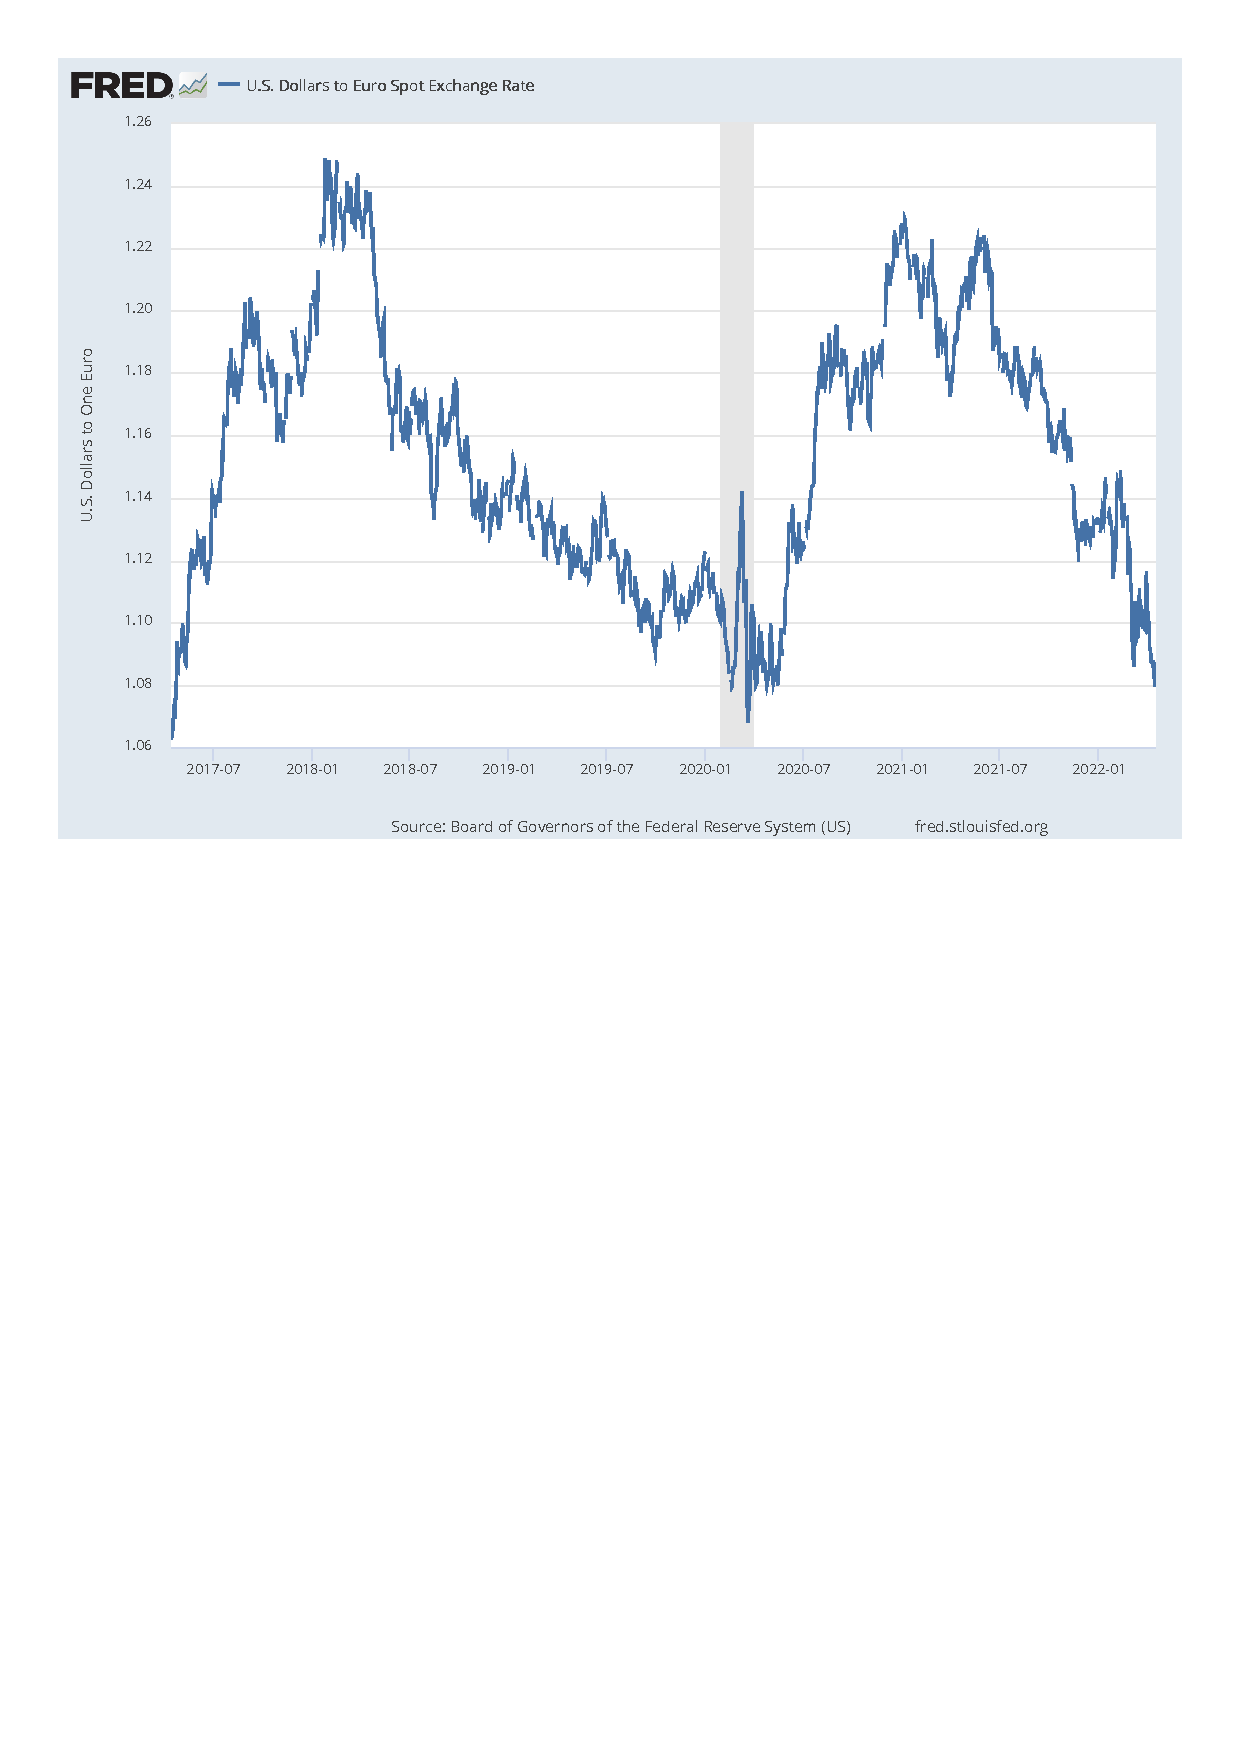
\includegraphics[trim=1cm 15.5cm 1cm 1cm,clip,width=6.5in]{figures/fred_usd_eur.pdf}

\vfill

\clearpage

\emph{For the following problems, please show your work and use the data above.}

\begin{enumerate}

\item How much did a bottle of French wine cost in U.S.~dollars in January 2021?

\vfill

\item How much did a bottle of French wine cost in U.S.~dollars in January 2022?

\vfill

\item How much did a bottle of French wine cost in U.S.~dollars in March 2018?

\vfill

\item Between March 2018 and January 2022, did the euro appreciate or depreciate relative to the dollar? Explain.

\vfill

\end{enumerate}

\end{document}
